\documentclass[12pt]{article}

\usepackage{dsfont}
\usepackage{amsmath, amssymb,amsthm}
\usepackage{bm}
\usepackage{cite}
\usepackage[dvipsnames]{xcolor}
\usepackage{comment}
\usepackage{geometry}
\geometry{hmargin=2.5cm,vmargin=2.5cm}
\usepackage{hyperref}
\hypersetup{
	colorlinks = true,
	citecolor = cyan,
	linkcolor = magenta,
	breaklinks = true,
	linktocpage
}

\usepackage{fancyhdr}
% Define a custom style specifically for the first page
\fancypagestyle{firstpage}{
    \fancyhf{} % Clear all headers and footers
    \fancyfoot[C]{\thepage}
    \fancyfoot[R]{\today} % Put the date in the right footer
    \renewcommand{\headrulewidth}{0pt} % Remove top line
}

\usepackage{mathtools}
\DeclarePairedDelimiter{\ceil}{\lceil}{\rceil}
\usepackage{tikz}
 \usepackage{pgfplots}
%\usepackage{refcheck}


\allowdisplaybreaks

\theoremstyle{definition}
\newtheorem{definition}{Definition}
\newtheorem{proposition}[definition]{Proposition}
\newtheorem{remark}[definition]{Remark}
\newtheorem{theorem}[definition]{Theorem}
\newtheorem{corollary}[definition]{Corollary}
\newtheorem{lemma}[definition]{Lemma}
\newtheorem{axiom}[definition]{Axiom}
\newtheorem{example}[definition]{Example}

%\counterwithin{equation}{section}

\newcommand{\D}[2]{\prescript{}{#1}{D}_x^{#2}}
\newcommand{\I}[2]{\prescript{}{#1}{I}_x^{#2}}

%%%%%
\begin{document}
%%%%%

\begin{center}
{\bf {\Large Introduction to Fractional Calculus}}\\[1cm]
\end{center}

In Calculus I and II we learn to compute integer value derivatives and integrals
\[
\cdots \longleftarrow \iiint f \longleftarrow \iint f \longleftarrow \int f \longleftarrow f \longrightarrow f^\prime \longrightarrow f^{\prime\prime} \longrightarrow f^{\prime\prime\prime} \longrightarrow \cdots
\]
Therefore, we know how to compute
%
\begin{equation}\label{Dn}
D^n[f(x)]\qquad n\;\in\; \mathbb{Z}
\end{equation}
%
where 
\[
D^{-1}[f(x)] = \int f(x)\, dx\qquad \text{and}\qquad D[f(x)] = \frac{df}{dx}
\]
A natural question is whether the integer $n$ in \eqref{Dn} can be replaced by
\[
D^\alpha[f(x)]\qquad\text{with}\qquad \alpha \in \mathbb{Q}\quad\text{or}\quad \alpha \in \mathbb{R}\quad\text{or}\quad \alpha \in \mathbb{C}?
\]
This is an old question that dates back to the foundations of Calculus.  Leibniz, who introduce both the $d^nf/dx^n$ and $\int f(x)\, dx$ notations, wrote in September of 1695 to his friend l'Hospital, \cite[p.\ 299]{M-1977}:
\begin{quote}
{\it ``Jean Bernoulli seems to have told you of me having mentioned to
him a marvelous analogy which makes it possible to say in
a way that successive differentials are in geometric progression.
One can ask what would be a differential having as its exponent
a fraction. You see that the result can be expressed by an infinite
series, although this seems removed from Geometry, which does not
yet know of such fractional exponents. It appears that one day these
paradoxes will yield useful consequences, since there is hardly a
paradox without utility. Thoughts that mattered little in themselves
may give occasion to more beautiful ones."}
\end{quote}
Thirty-five years later, Euler expressed a similar thought, and took explicit note of the fact that a kind of interpolation theory comes necessarily into play, \cite{W-1997}:
\begin{quote}
{\it ``Concerning transcendental progressions whose terms cannot be
given algebraically: when $n$ is a positive integer, the ratio $d^nf/dx^n$
can always be expressed algebraically. Now it is asked: what kind of ratio can be made if $n$ be a fraction? $\ldots$ the matter may be expedited
with the help of the interpolation of series, as explained earlier in
this dissertation."}
\end{quote}

The answer to our question is yes, and we first begin by extending the definition of iterated integrals
\[
D^{-n}[f(x)] = \int_a^x \int_a^{x_1}\int_a^{x_2}\cdots\int_a^{x_{n-1}} f(x_n)\; dx_n \cdots dx_2\, dx_1,
\]
where $n \in \mathbb{N}$.

\begin{theorem}[Cauchy's formula for repeated integrals]
Let $f(x)$ be continuous on $[a,x]$ and $n\in \mathbb{N}$, then
%
\begin{equation}\label{cauchy formula}
\int_a^x \int_a^{x_1}\int_a^{x_2}\cdots\int_a^{x_{n-1}} f(x_n)\; dx_n \cdots dx_2\, dx_1 = \frac{1}{(n-1)!} \int_a^x (x-t)^{n-1} f(t)\, dt.
\end{equation}
\end{theorem}

\begin{proof}
We prove equality \eqref{cauchy formula} using induction.  For the base case $n=1$, starting from the right hand side we have
\[
\frac{1}{(1-1)!} \int_a^x (x-t)^0 f(t)\, dt = \int_a^x f(t)\, dt = \int_a^x f(x_1)\, dx_1.
\]
For a fixed $n\in \mathbb{N}$, we assume that \eqref{cauchy formula} holds.  For $n+1$,
%
\begin{align*}
\int_a^x\bigg[\int_a^{x_1}\cdots \int_a^{x_n} f(x_{n+1})\, dx_{n+1}\cdots dx_2\bigg] dx_1 &= \int_a^x \frac{1}{(n-1)!} \int_a^s (s-t)^{n-1} f(t)\, dt ds \\
&=\frac{1}{(n-1)!} \int_a^x \int_a^s (s-t)^{n-1} f(t)\, dt ds
 \\
\end{align*}
where $s=x_1$.  The domain of integration is
%
\begin{center}
\begin{tikzpicture}[
    >=stealth,
    line cap=round,
    line join=round,
    scale=1
]

%------------------------------------------------
% Axes
%------------------------------------------------
\draw[->, thick] (-0.35,0) -- (6,0)
    node[right] {$s$};

\draw[->, thick] (0,-0.35) -- (0,5.5)
    node[right] {$t$};

%------------------------------------------------
% Tick marks and labels on s-axis
%------------------------------------------------
\draw[thick] (2.0,-0.12) -- (2.0,0.12);
\node[below=5pt] at (2.0,0) {$a$};

\draw[thick] (4.9,-0.12) -- (4.9,0.12);
\node[below=5pt] at (4.9,0) {$x$};

%------------------------------------------------
% Tick marks and labels on t-axis
%------------------------------------------------
\draw[thick] (-0.12,2.0) -- (0.12,2.0);
\node[left=7pt] at (0,2.0) {$a$};

\draw[thick] (-0.12,4.35) -- (0.12,4.35);
\node[left=7pt] at (0,4.35) {$x$};

%------------------------------------------------
% Dashed diagonal t=s
%------------------------------------------------
\draw[
    thick,
    dashed,
    dash pattern=on 7pt off 8pt
] (-0.55,-0.55) -- (5.55,5.55)
    node[right=2pt] {$t=s$};

%------------------------------------------------
% Rectangular/step-like region
%------------------------------------------------

% bottom horizontal segment
\draw[thick] (2,2) -- (4.9,2);

% right vertical side
\draw[thick] (4.9,2) -- (4.9,4.9);

% horizontal upper segment
%\draw[thick] (3.0,3.15) -- (4.9,3.15);

% small vertical segment
%\draw[thick] (3.0,1.45) -- (3.0,3.15);

%------------------------------------------------
% Small rectangular band at the upper horizontal
%------------------------------------------------
\draw[thick]
    (3.35,3.15) rectangle (4.9,3.38);

%------------------------------------------------
% Small vertical band
%------------------------------------------------
\draw[thick]
    (3,2) rectangle (3.24,3);

\end{tikzpicture}
\end{center}
%
where we integrate over the domain using vertical infinitesimal rectangles. We change the order of integration and integrate using horizontal infinitesimal rectangles so that
%
\begin{align*}
\frac{1}{(n-1)!}\int_a^x \int_a^s (s-t)^{n-1} f(t)\, dt ds
&= \frac{1}{(n-1)!}\int_a^x  \int_t^x (s-t)^{n-1} f(t)\, ds dt \\
&= \frac{1}{(n-1)!}\int_a^x f(t) \bigg[\int_t^x (s-t)^{n-1} f(t)\, ds\bigg] dt \\
&= \frac{1}{(n-1)!} \int_a^x f(t)\bigg[\frac{(s-t)^n}{n}\bigg]^x_t dt \\
&= \frac{1}{n!} \int_a^x (x-t)^n f(t)\, dt.
\end{align*}
\end{proof}

To extend the notion of iterated integral from $n \in \mathbb{N}$ to $\alpha \in \mathbb{C}$, we need to introduce the \emph{gamma function}.   The gamma function $\Gamma(z)$ is defined for all complex numbers $z$ except non-positive integers.  For $z \in \mathbb{C}$ with $\mathfrak{R}(z)>0$, the gamma function is defined by the improper integral
\[
\Gamma(z) = \int_0^\infty t^{z-1}e^{-t}\, dt.
\]
The function is extended to complex numbers $z$ with negative real part using the identity
\[
\Gamma(z+1) = z\, \Gamma(z).
\]
Indeed, using integration by parts using $u=t^z$ and $dv = e^{-t}\, dt$ we have that 
%
\begin{align*}
\Gamma(z+1) &= \int_0^\infty t^z e^{-t} dt = \big[-t^ze^{-t}\big]_0^\infty + \int_0^\infty z t^{z-1}e^{-t}\, dt\\
&= z \int_0^\infty t^{z-1} e^{-t}\, dt = z\, \Gamma(z).
\end{align*}

With 
\[
\Gamma(1) = \int_0^\infty t^{1-1}e^{-t}\, dt = \int_0^\infty e^{-t}\,dt = \big[-e^{-t}\big]_0^\infty = 1
\]
we find that for $n \in \mathbb{N}$
\[
\Gamma(n+1) = n\cdot \Gamma(n) = n(n-1)\cdot\Gamma(n-2) = \cdots
= n(n-1)\cdots 2\cdot \Gamma(1) = n(n-1)\cdots 2\cdot 1 = n!
\]

\begin{definition}
The Riemann--Liouville fractional integral for \footnote{More generally $\alpha \in \mathbb{C}$ with $\mathfrak{R}(\alpha)>0$, but we don't consider this more general case in these notes.} $\alpha >0$ is given by
%
\begin{equation}\label{I}
\I{a}{\alpha} f(x) = \frac{1}{\Gamma(\alpha)}\int_a^x(x-t)^{\alpha-1} f(t)\, dt,
\end{equation}
%
which is obtained by replacing
\[
n \to \alpha \qquad \text{and}\qquad (n-1)! \to \Gamma(n) \to \Gamma(\alpha)
\]
in \eqref{cauchy formula}.
\end{definition}

\begin{proposition}
The power rule for the Riemann--Liouville fractional integral is
%
\begin{equation}\label{power rule}
\I{0}{\alpha}[x^\nu] = \frac{\Gamma(\nu+1)}{\Gamma(\nu+\alpha+1)} x^{\nu+\alpha}.
\end{equation}
\end{proposition}

\begin{proof}
Using the definition of the Riemann--Liouville fractional integral
\[
\I{0}{\alpha} = \frac{1}{\Gamma(\alpha)}\int_0^x (x-u)^{\alpha-1} u^\nu\, du.
\]
We make the change of variable $u = xt$ so that $t= \dfrac{u}{x}$ and $du = x\, dt$.  The integral becomes
%
\begin{align*}
\frac{1}{\Gamma(\alpha)}\int_0^x (x-u)^{\alpha-1} u^\nu\, du 
&= \frac{1}{\Gamma(\alpha)} \int_0^1 (x-xt)^{\alpha-1}(xt)^\nu x\, dt \\
&= \frac{1}{\Gamma(\alpha)} \int_0^1 x^{\alpha-1}(1-t)^{\alpha-1} x^\nu t^\nu x\, dt \\
&= \frac{x^{\alpha+\nu}}{\Gamma(\alpha)} \int_0^1 (1-t)^{\alpha-1} t^\nu\, dt.
\end{align*}
Using the Euler Beta function
\[
B(p,q) = \int_0^1 t^{p-1}(1-t)^{q-1} dt = \frac{\Gamma(p)\Gamma(q)}{\Gamma(p+q)}
\]
the last integral equals
\[
\frac{x^{\alpha+\nu}}{\Gamma(\alpha)} \int_0^1 (1-t)^{\alpha-1} t^\nu dt 
= \frac{x^{\alpha+\nu}}{\Gamma(\alpha)} B(\nu+1,\alpha) 
= \frac{x^{\alpha+\nu}}{\Gamma(\alpha)}\cdot \frac{\Gamma(\nu+1)\Gamma(\alpha)}{\Gamma(\alpha+\nu+1)} 
= \frac{\Gamma(\nu+1)}{\Gamma(\alpha+\nu+1)} x^{\alpha+\nu}.
\]
\end{proof}

\begin{example}
Using \eqref{power rule}
\[
\I{0}{1/2}[x] = \frac{\Gamma(2)}{\Gamma(2+1/2)} x^{3/2}
\]
Using $\Gamma(2) = 1! = 1$ and
\[
\Gamma(5/2) = \Gamma(3/2+1) = \frac{3}{2}\, \Gamma(3/2) = \frac{3}{2}\cdot \frac{1}{2}\, \Gamma(1/2) = \frac{3}{4}\sqrt{\pi},
\]
we find that
\[
\I{0}{1/2}[x] = \frac{1}{\frac{3}{4}\sqrt{\pi}} x^{3/2} = \frac{4x^{3/2}}{3\sqrt{\pi}}.
\]
Next,
\[
\I{0}{1/2}[x^{3/2}] = \frac{\Gamma(5/2)}{\Gamma(3)} x^2 = \frac{\frac{3}{4}\sqrt{\pi}}{2} x^2
\]
Thus,
\[
\I{0}{1/2} \I{0}{1/2}[x] = \frac{x^2}{2} = \I{0}{1}[x] = \int_0^x t\, dt.
\]
\begin{center}
\vspace{0.25cm}
\href{https://www.desmos.com/calculator/vpzhtosg3n}{{\bf {\Large Desmos Animation}}}
\vspace{0.25cm}
\end{center}
\end{example}

It would be tempting to extend the notion of fractional integral by allowing $\alpha$ in \eqref{I} to be negative.  Unfortunately, this is not possible as the $\Gamma$ function is undefined at negative integers, as it can be seen from its graph.
\begin{center}
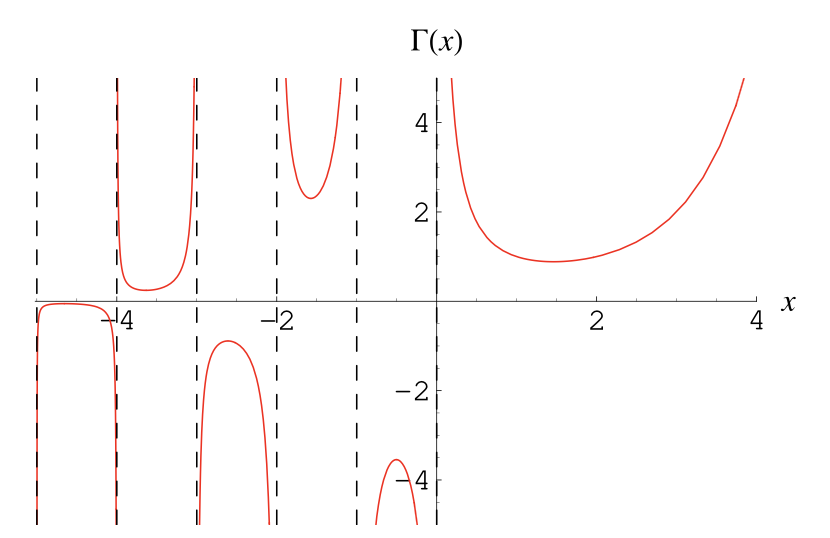
\includegraphics[scale=0.6]{../figures/gamma.png}
\end{center}

To introduce the notion of fractional derivative, we extend the property that differentiation and integration cancel in ``integer" calculus so that 
\[
\D{a}{n} \circ \I{a}{m} [f(x)] = \D{a}{n-m}[f(x)]
\]
when $n,m\in \mathbb{N}$.  Thus, to define, for example, the half derivative we use
\begin{align*}
\D{a}{1/2}[f(x)] &= \D{a}{1} \circ \I{a}{1/2}[f(x)] \\
&= \frac{d}{dx}\bigg[\frac{1}{\Gamma(1/2)} \int_a^x(x-t)^{-1/2}f(t)\, dt \bigg].
\end{align*}

\begin{example}
Computing the half derivative of $x^2$ we obtain
\[
\D{0}{1/2}[x^2] = \frac{d}{dx}\big(\I{0}{1/2}[x^2]\big) =
 \frac{d}{dx}\bigg(\frac{\Gamma(3)}{\Gamma(7/2)}x^{5/2}\bigg) 
= \frac{5\, \Gamma(3)}{2\, \Gamma(7/2)} x^{3/2} = \frac{5}{\frac{15\sqrt{\pi}}{8}} x^{3/2} = \frac{8 x^{3/2}}{3\sqrt{\pi}}.
\]
Differentiating the result obtained
\[
\D{0}{1/2}\bigg[\frac{8 x^{3/2}}{3\sqrt{\pi}}\bigg] = 
\frac{8}{3\sqrt{\pi}} \frac{d}{dx}\big(\I{0}{1/2}[x^{3/2}]\big)
=\frac{8}{3\sqrt{\pi}} \cdot \frac{\frac{3}{4}\sqrt{\pi}}{2} \frac{d}{dx}(x^2) = 2 x.
\]
As expected,
\[
\D{0}{1/2}\circ \D{0}{1/2} = \D{0}{1} = \frac{d}{dx}.
\]
\end{example}

\begin{definition}
For $\alpha \in \mathbb{R}$, the Riemann--Liouville fractional derivative of $f(x)$ is given by
\[
\D{a}{\alpha}[f(x)] = \begin{cases}
\bigg(\dfrac{d}{dx}\bigg)^{\ceil{\alpha}} \I{a}{\ceil{\alpha}-\alpha} [f(x)] & \text{if } \alpha > 0 \\
\hspace*{1.5cm} f(x) & \text{if } \alpha =0 \\
\hspace*{1cm} \I{a}{-\alpha}[f(x)] &\text{if }\alpha < 0
\end{cases}
\]
\end{definition}

\begin{proposition}
The Riemann--Liouville fractional derivative of the monomial $x^\nu$ is
%
\begin{equation}\label{fder monomial}
\D{0}{\alpha}[x^\nu] =
\frac{\Gamma(\nu+1)}{\Gamma(\nu - \alpha + 1)} x^{\nu-\alpha}.
\end{equation}
\end{proposition}

\begin{proof}
For $\alpha > 0$ we have
\begin{align*}
\D{0}{\alpha}[x^\nu] &= \bigg(\dfrac{d}{dx}\bigg)^{\ceil{\alpha}} \I{a}{\ceil{\alpha}-\alpha} [x^\nu] = \bigg(\dfrac{d}{dx}\bigg)^{\ceil{\alpha}}\bigg[\frac{\Gamma(\nu+1)}{\Gamma(\nu+ \ceil{\alpha}-\alpha+1)} x^{\nu+\ceil{\alpha}-\alpha}\bigg] \\
&= \frac{\Gamma(\nu+1)}{\Gamma(\nu+ \ceil{\alpha}-\alpha+1)} \bigg(\dfrac{d}{dx}\bigg)^{\ceil{\alpha}}(x^{\nu+\ceil{\alpha}-\alpha}) \\
&= \frac{\Gamma(\nu+1)}{\Gamma(\nu+ \ceil{\alpha}-\alpha+1)} (\nu+\ceil{\alpha}-\alpha)(\nu+\ceil{\alpha}-\alpha-1)\cdots(\nu+1-\alpha)\; x^{\nu-\alpha}\\
&= \frac{\Gamma(\nu+1)}{\Gamma(\nu-\alpha+1)} x^{\nu-\alpha},
\end{align*}
where in the last equality we used the identity
\[
\Gamma(z+1) = z\, \Gamma(z) = \frac{\Gamma(z+n+1)}{(z+1)(z+2)\cdots(z+n)}
\]
with $z=\nu-\alpha$ and $n = \ceil{\alpha}$.

When $\alpha=0$, the right hand side of \eqref{fder monomial} reduces to
\[
\frac{\Gamma(\nu+1)}{\Gamma(\nu + 1)} x^{\nu} = x^\nu = \D{0}{0}[x^\nu].
\]
When $\alpha<0$ we have
\[
\D{0}{\alpha}[x^\nu] = \I{a}{-\alpha}[x^\nu] = \frac{\Gamma(\nu+1)}{\Gamma(\nu-\alpha+1)} x^{\nu-\alpha}
\]
using \eqref{power rule}.
\end{proof}

With the fractional derivative being an interpolation between integer derivatives, there are many ways to interpolate and not surprisingly, there are different definition of fractional derivative.  Another widely used definition is the Caputo fractional derivative.

\begin{definition}
The Caputo fractional derivative is given by
\[
\D{a}{\alpha}[f(x)] = \frac{1}{\Gamma(\ceil{\alpha}-\alpha)}\int_a^x(x-t)^{\ceil{\alpha}-\alpha-1}f^{(\ceil{\alpha})}(t)\, dt.
\]
\end{definition}

The main difference between the Caputo and Riemann--Liouville fractional derivatives are the order in which one differentiates and integrates.  For the Riemann--Liouville fractional derivative, one integrates first and then differentiates while the order is inverted in the Caputo fractional derivative. the Caputo fractional derivative is preferred when modeling real-world physical systems.  On the other hand, the Riemann--Liouville fractional derivative is easier to analyze mathematically and build theoretical frameworks around as it requires fewer smoothness restrictions on the function $f(t)$.



\begin{thebibliography}{99}
\bibitem{M-1977} 
Mandelbrot, B., {\it Fractals: Form, Chance, and Dimension}, 1977.

\bibitem{W-1997}
Wheeler, N., Construction \& physical application of the fractional calculus, notes, 1997.
\end{thebibliography}

\end{document}